\documentclass[a4paper, 12pt]{article}

% Работа с русским языком
\usepackage{cmap}
\usepackage{mathtext}
\usepackage[T2A]{fontenc}
\usepackage[utf8]{inputenc}
\usepackage[english,russian]{babel}

% Математика и графика
\usepackage{amsmath,amsfonts,amssymb,amsthm,mathtools}
\usepackage{icomma}

\usepackage{physics}
\usepackage{graphicx}
\usepackage{calc}
\usepackage{wrapfig}
\usepackage{setspace}
\usepackage{indentfirst}
\usepackage{gensymb}
\usepackage{longtable}
\usepackage{float}
\usepackage{multirow}
\setlength{\textfloatsep}{10pt}

% Точка после секции
\usepackage{titlesec}
\titlelabel{\thetitle.\quad}

\usepackage[left=25mm, top=14mm, right=25mm, bottom=30mm, nohead]{geometry}
\usepackage{fancybox,fancyhdr} 
\setcounter{page}{1} % счетчик нумерации страниц
\headsep=10mm 
\usepackage{xcolor}
\usepackage{hyperref} 
\hypersetup{colorlinks=true, allcolors=[RGB]{010 090 200}} % цвет ссылок 
\newcommand{\lr}[1]{\left({#1}\right)} % команда для скобок
\newcommand{\te}[2]{{#1}_{\text{#2}}}


\begin{document}

\begin{titlepage}
        %\setlength{\parindent}{0pt}
        %\vspace*{-3.8\baselineskip}
        \begin{center}
            %\includegraphics[width=0.2\linewidth]{logo.png}\\[1ex]
		{\large МОСКОВСКИЙ ФИЗИКО-ТЕХНИЧЕСКИЙ ИНСТИТУТ (НАЦИОНАЛЬНЫЙ ИССЛЕДОВАТЕЛЬСКИЙ УНИВЕРСИТЕТ)}
		{\large Физтех-школа физики и исследований им. Ландау}
	\end{center}
	
	
	\vspace{4.5cm}
	{\huge
		\begin{center}
			Отчет по лабораторной работе №3.2.5 \\
                \textbf{Свободные и вынужденные колебания в электрическом контуре}\\
		\end{center}
	}
	\vspace{2cm}
	\begin{flushright} % выравнивание по правому краю
		\begin{minipage}{0.3\textwidth} % врезка в половину ширины текста
			\begin{flushleft} % выровнять её содержимое по левому краю

				\large\textbf{Работу выполнил:}\\
				\large {Комкин Михаил Валерьевич} \\
				\large {Группа: Б01-303} \\

			\end{flushleft}
		\end{minipage}
	\end{flushright}
	\vspace{8cm}
	\begin{center}
            
		Долгопрудный 2024
	\end{center}
\end{titlepage}

\textbf{Цель работы:}
Исследование свободных и вынужденных колебаний в колебательном контуре.

\section{Теоретические сведения:}

{\bf 1) Введение}

Рассмотрим $RLC$--контур. Запишем II правило Киргхофа:
\begin{figure}[h!]
    \centering
    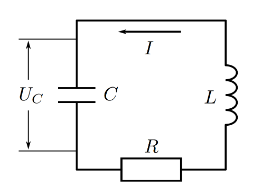
\includegraphics[scale = 0.5]{LCR.png}
    \caption{LCR--контур}
\end{figure}

$$I R + U_C + L \dot{I} = 0 \eqno{(1)}$$
Так как $U_C = \frac{q}{C}$ и $I = \dot{q}$, то
$$CL \dfrac{\mathrm{d}^2 U_C}{\mathrm{d} t^2} + C R \dfrac{\mathrm{d} U_C}{\mathrm{d} t} + U_C = 0 \eqno{(2)}$$
Введем обозначения:
$$\gamma = \dfrac{R}{2L} - \text{ коэффициент затухания}$$
$$\omega_0^2 = \dfrac{1}{LC} - \text{ собственная круговая частота}$$
$$T_0 = \dfrac{2 \pi }{\omega_0} = 2 \pi \sqrt{LC} - \text{период собственных колебаний}$$
Тогда уравнение (2) принимает вид:
$$\ddot{U}_C + 2 \gamma \dot{U}_C + \omega_0^2 U_C = 0 \eqno{(3)}$$

{\bf 2) Затухающие колебания ($0 < \gamma < \omega_0)$}

Отметим, что условие возникновения этого режима можем переписать в виде:
$$0 < R < 2 \sqrt{\dfrac{L}{C}} = R_{\text{кр}} \eqno{(4)}$$

При таком соотношении параметров решение будет иметь вид:

$$U_C(t) = U_0 e^{- \gamma t} \cos{(\omega_1 t + \varphi_0)} \eqno{(5)}$$
где $U_0$ и $\varphi_0$ -- константы, определяемые из начальных условий, а
$$\omega_1 = \sqrt{\omega_0^2 - \gamma^2} \eqno{(6)}$$
называется круговой частотой свободных затухающих колебаний.

Представим решение в другом виде:
$$U_C(t) = e^{-\gamma t} ( a \cos{(\omega_1 t)} + b \sin{(\omega_1 t)}) \eqno{(7)}$$
Так как $I = \dot{q} = C \dot{U_C}$, то
$$I(t) = С  e^{-\gamma t} ( (b \omega_1 - a \gamma) \cos{(\omega_1 t)} - (b \gamma + a \omega_1) \sin{(\omega_1 t)}) \eqno{(8)}$$
Из формул (7) и (8) следует параметрическое представление траектории системы на фазовой плоскости переменных ($U_C$, $I$). 

\begin{figure}[h!]
    \centering
    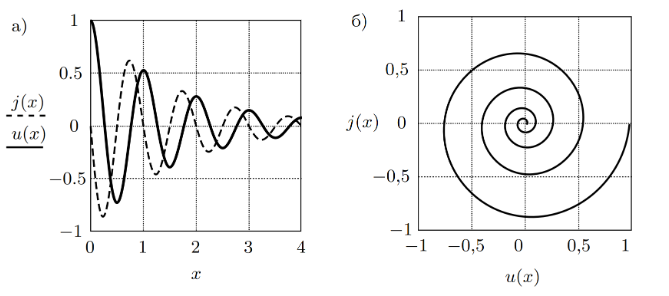
\includegraphics[scale = 0.25]{затух затух.png}
    \caption{a) ток в контуре $j(x)$ и напряжение на конденсаторе $u(x)$} б) траектория системы на фазовой плоскости $j(u)$
\end{figure}

На рис. 2 представлены в безразмерных переменных зависимости напряжения и тока в контуре от времени в режиме свободных затухающих колебаний.

{\bf 3) Характеристики затухающих колебаний}

Из формулы (5) видно, что затухающие колебания напряжения не являются, периодическими функциями времени. Однако эти величины дважды за время
$$T_1 = \dfrac{2\pi}{\omega_1} = \dfrac{T_0}{\sqrt{1- \frac{\gamma^2}{\omega_0^2}}} \eqno{(9)}$$
проходят через 0. Также это период между двумя последовательными максимумами/минимумами $U_C(t)$ и $I(t)$. $T_1$ называется периодом затухающих колебаний.

В качестве характеристик процесса затухания колебаний помимо коэффициента затухания $\gamma$ используют характерное время затухания:
$$\tau = \dfrac{1}{\gamma} = \dfrac{2 L}{R} \eqno{(10)}$$
и логарифмический декремент:
$$\Theta = \ln({\dfrac{U_k}{U_{k+1}}}) = \gamma T_1 \eqno{(11)}$$
где $U_k$ и $U_{k+1}$ --  два последовательных максимальных отклонения рассматриваемой величины.

Обозначим $N_{\tau}$ -- число полных колебаний за время затухания $\tau$. Тогда можем выразить $\Theta$ ещё одним способом:
$$\Theta = \dfrac{1}{N_{\tau}} \eqno{(12)}$$
На практике удобнее использовать отношение максимальных отклонений, разделённых целым числом $n$ периодов $T_1$:
$$\Theta = \dfrac{1}{n}  \ln({\dfrac{U_k}{U_{k+n}}}) \eqno{(13)}$$

С логарифмическим декрементом связана ещё одна важнейшая характеристика колебательного
контура -- добротность $Q$. По определению:
$$Q = \dfrac{\pi}{\Theta} = \dfrac{\pi}{\gamma T_1}= \dfrac{1}{2}\sqrt{\dfrac{\omega_0^2}{\gamma^2} - 1} = \dfrac{1}{2}\sqrt{\dfrac{R_{\text{кр}}}{R^2} - 1} \eqno{(14)}$$

Добротность обладает энергетическим смыслом. Пусть $Q \gg 1$. Обозначим $W$ -- запасенная в системе энергия, $\Delta W$ -- её потери за период. В моменты когда $U_C$ -- максимально, вся энергия сосредоточена в конденсаторе. Отсюда:
$$W = \dfrac{1}{2} C U_C^2(t) = \dfrac{1}{2} C U_0^2 e^{-2 \gamma t} \eqno{(15)}$$
$$\Delta W = \dfrac{1}{2} C U_0^2 e^{-2 \gamma t} - \dfrac{1}{2} C U_0^2 e^{-2 \gamma (t + T)}\approx 2\gamma T_1 W \eqno{(16)}$$
Из формул (14) - (16) получаем:
$$Q = 2\pi \dfrac{W}{\Delta W} \approx \dfrac{\omega_0^2}{2 \gamma}$$

{\bf 4) Критический режим $(\gamma = \omega_0)$}

В этом случае $R = R_{\text{кр}}$, а решение уравнения (3) имеет вид:
$$U(t) = (a_1 + b_1 t) e^{-\gamma t}$$
где $a_1$ и $b_1$ -- постоянные интегрирования, определяемые из начальных условий.

{\bf 5) Апериодический режим $(\gamma > \omega_0)$}

В этом режиме $R > R_{\text{кр}}$ и решение (3) имеет вид:

$$U_C = e^{-\gamma t} (b_1 e^{\alpha t} + b_2 e^{- \alpha t})$$

Графики, а также фазовая траектория системы в апериодическом режиме показаны в безразмерных переменных на рис.3

\begin{figure}[h!]
    \centering
    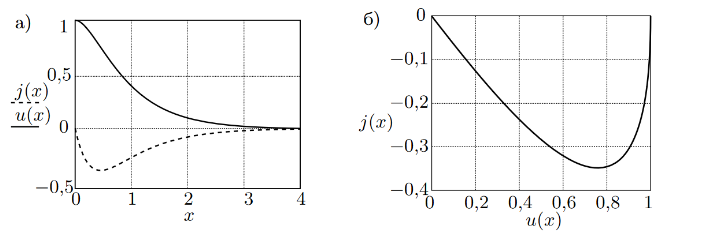
\includegraphics[scale = 0.3]{апериод.png}
    \caption{a) ток в контуре $j(x)$ и напряжение на конденсаторе $u(x)$} б) траектория системы на фазовой плоскости $j(u)$
\end{figure}

Нетрудно показать, что в этом режиме при любых начальных условиях система стремится к равновесному состоянию $U_C = 0$, $I = 0$.
При этом возможно не более одного прохождения через экстремальное состояние, и не более одного — через равновесное.

\section{Экспериментальная установка:}

Колебательный контур состоит из постоянной индуктивности $L$ с активным сопротивлением $R_L$, переменной емкости $C$ и сопротивления $R$. Картина колебаний
напряжения на емкости наблюдается на экране двухканального осциллографа. Для возбуждения затухающих колебаний используется генератор сигналов специальной
формы. Сигнал с генератора поступает через конденсатор $C_1$ на вход колебательного контура. Данная емкость необходима чтобы выходной импеданс генератора был
много меньше импеданса колебательного контура и не влиял на процессы, проходящие в контуре.

\begin{figure}[h]
    \centering
    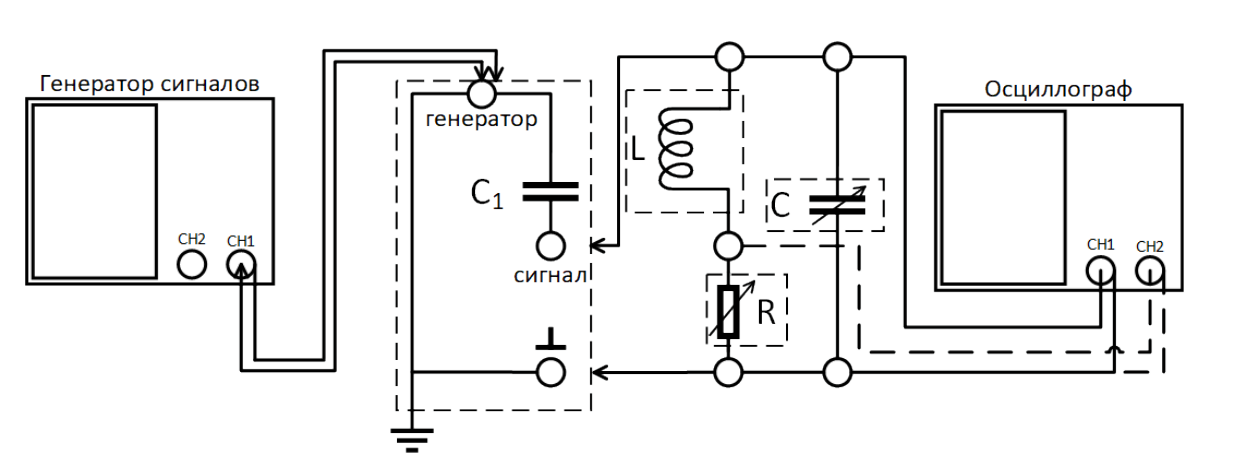
\includegraphics[width=0.5\linewidth]{ust.png}
    \caption{Схема установки для исследования вынужденных колебаний}
\end{figure}

Установка предназначена для исследования не только возбужденных, но и свободных колебаний в электрической цепи. При изучении свободно затухающих колебаний генератор специальных сигналов на вход колебательного контура подает периодические короткие импульсы, которые заряжают конденсатор $C$. За время между
последовательными импульсами происходит разрядка конденсатора через резистор
и катушку индуктивности. Напряжение на конденсаторе $U_C$ поступает на вход канала $1(X)$ электронного осциллографа. Для наблюдения фазовой картины затухающих
колебаний на канал $2(Y)$ подается напряжение с резистора $R$ (пунктирная линия на схеме установки), которое пропорционально току $I (I \propto \mathrm{d}U_C/\mathrm{d}t)$.

При изучении возбужденных колебаний на вход колебательного контура подается синусоидальный сигнал. С помощью осциллографа возможно измерить зависимость амплитуды возбужденных колебаний в зависимости от частоты внешнего сигнала, из которого возможно определить добротность колебательного контура. Альтернативным способом расчета добротности контура является определение декремента затухания по картине установления возбужденных колебаний. В этом случае генератор сигналов используется для подачи цугов синусоидальной формы.


\section{Результаты измерений и обработка данных:}
\subsection{Подготовка приборов к работе:}
\textbf{1.} Подключим генератор специальных сигналов к входу 1(X) осциллографа. Установим на генераторе последовательность импульсов длительностью (PullWidth) 10 мкс, с частотой повторения импульсов
$\nu = 100$ Гц, а амплитуду сигнала 20 В. 

\textbf{2.} Убедимся, что на экране осциллографа отображаются периодические импульсы, и приступим к сборке схемы.

\subsection{Измерение периодов свободных колебаний:}
\textbf{1.} Установим на магазине сопротивлений величину $R = 0$ Ом,на магазине индуктивностей $L = 100$ мГн, на магазине емкостей величину $C = 0$ мкФ. Из-за наличия минимального значения ёмкости $C_0$ в контуре реализуются свободные колебания. Получим изображение этих затухающих свободных колебаний на экране осциллографа.


\textbf{2.} C помощью кнопки "Cursor" на осциллографе измерим период свободных колебаний и по нему определим нулевую ёмкость $C_0$ по формуле:
\[
	C_0 = \frac{{\frac{T_0}{2\pi}}^2}{L}
\]

Полученный период $T_0 = (68,4 \pm 0,3)$ мкс, следовательно, $C_0 = (1,19 \pm 0,01)$ нФ

\textbf{3.} Изменяя ёмкость от 0 мкФ до 0.009 мкФ проведём измерения
периодов и занесём результаты в таблицу 1:
\begin{table}[h!]
\centering
\caption{Зависимость периода свободных колебаний от ёмкости конденсатора}
\vspace{0.3cm}
\label{tab:1}
\begin{tabular}{|c|c|c|}
\hline
С, нФ & $\te{T}{эксп}$, мкс & $\te{T}{теор}$, мкс \\ \hline
2,2   & 92                & 93                \\ \hline
3,2   & 112               & 112               \\ \hline
4,2   & 130               & 129               \\ \hline
5,2   & 143               & 143               \\ \hline
6,2   & 157               & 156               \\ \hline
7,2   & 170               & 169               \\ \hline
8,2   & 180               & 180               \\ \hline
9,2   & 190               & 191               \\ \hline
10,2  & 201               & 201               \\ \hline
\end{tabular}
\end{table}
Построим график зависимости $T_\text{эксп}(T_{\text{теор}})$
\begin{figure}[h!]
	\begin{center}
	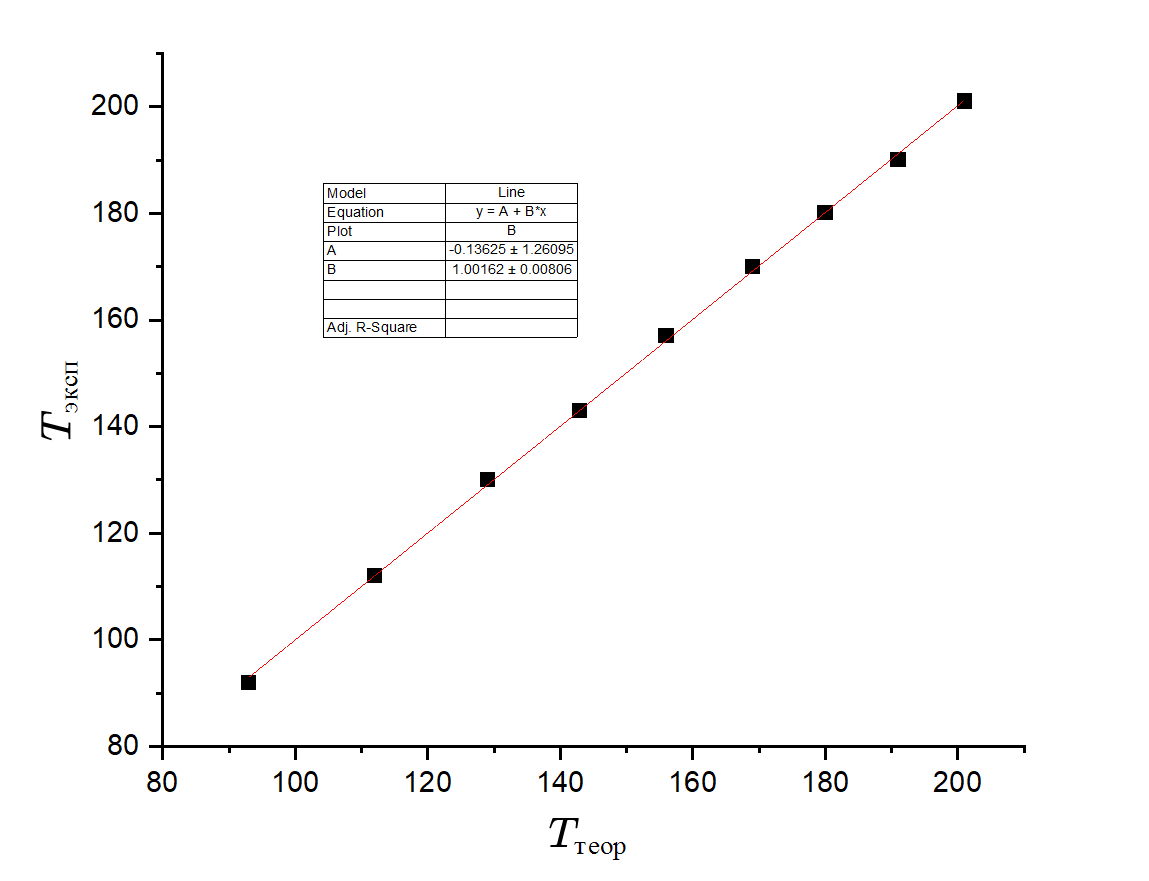
\includegraphics[width=\textwidth]{image.png}
	\caption{Зависимость $T_{\text{эксп}}(T_{\text{теор}})$} \
	\end{center}
	\end{figure}
$$k = (1,00 \pm 0.01)$$


\newpage
\subsection{Критическое сопротивление и декремент затухания:}

\textbf{1.} Приняв $L = 100$ мГн, рассчитаем ёмкость $C^*$, при которой собственная частота колебаний $\nu_0$ составляет $6,5$ кГц.
$$C^* = \frac{1}{L(2\pi \nu_0)^2}$$
Для выбранных $L$ и $C^*$ рассчитаем критическое сопротивление контура $R_{cr}$ по формуле
$$R_{cr} = 2\sqrt{\frac{L}{C^*}}$$
Полученные значения:
$$C^* = 6 \text{ нФ} \;\;\; R_{cr} = 8168 \text{ Ом}$$

\textbf{2.} Установим на магазине емкость, близкую к рассчитанной критической ($R_{cr} = 8168$ Ом). Увеличивая сопротивление R от нуля до Rcr, определим сопротивление магазина, при котором колебательный режим переходит в апериодический. Это происходит при значении $R \approx 5100$ Ом.

\textbf{3.} Будем устанавливать значения $R$ в контуре в интервале $(0,05-0,25)R_{cr}$. После, по полученной на осциллографе картине затухающих колебаний, измерим амплитуды, разделенные целым числом периодов $n$, и рассчитаем логарифмический декремент затухания по формуле:

$$\Theta = \frac{1}{n}\ln{\frac{U_m}{U_{m+n}}}$$
$$\sigma_\Theta = \frac{\sigma_U}{U_m} +  \frac{\sigma_U}{U_{m+n}}; \;\; \sigma_U = 1 \text{ мВ}$$
Результаты измерений заносим в таблицу:

\begin{table}[h]
\centering
\caption{Зависимость декремента затухания $\Theta$ от сопротивления}
\vspace{0.3cm}
\label{tab:2}
\begin{tabular}{|c|c|c|c|c|}
\hline
$R$, Ом & $U_1$, мВ & $U_2$, мВ & n  & $\Theta$ \\ \hline
60,7      & 872       & 216       & 14 & 0,100    \\ \hline
90,7      & 860       & 140       & 15 & 0,121    \\ \hline
120,7     & 840       & 104       & 15 & 0,139    \\ \hline
150,7     & 828       & 76        & 15 & 0,159    \\ \hline
180,7     & 812       & 56        & 15 & 0,178    \\ \hline
210,7     & 800       & 40        & 15 & 0,200    \\ \hline
\end{tabular}
\end{table}

Построим график, откладывая по оси абсцисс величину $R$, а по оси ординат величину $\Theta$ 





\textbf{4.} Построим график в координатах, откладывая по оси абсцисс величину $1/R^2$, а по оси ординат величину $1/\Theta^2$ (Рис. \ref{G3}).

\begin{figure}[!h]
\begin{center}
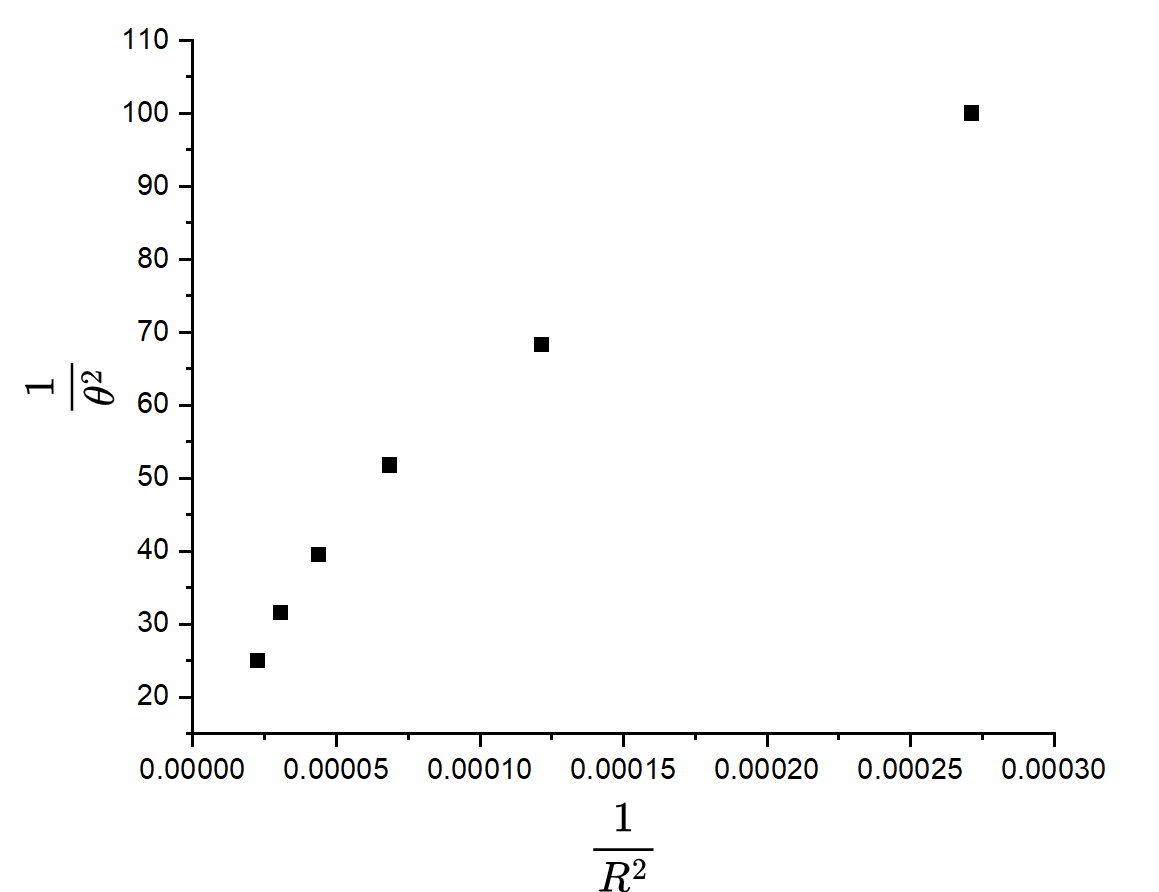
\includegraphics[width=\textwidth]{G3.png}
\caption{Зависимость $1/\Theta^2(1/R^2)$} \label{G3}
\end{center}
\end{figure}

\begin{figure}[h!]
\begin{center}
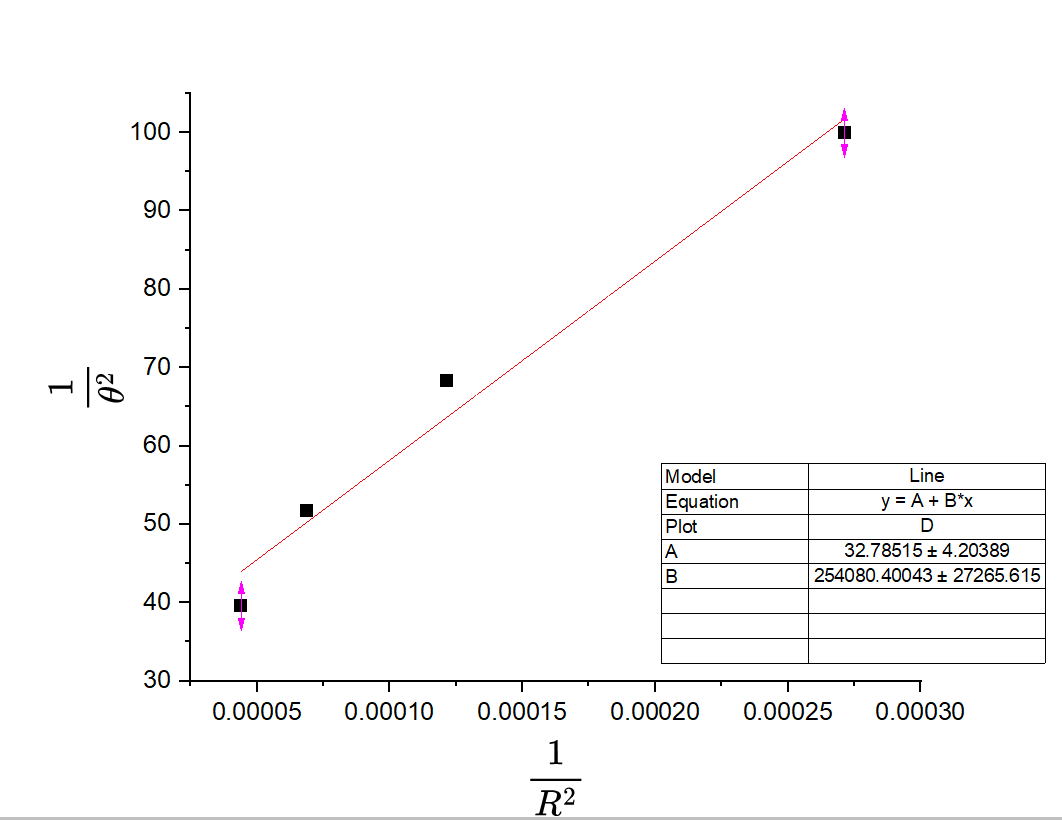
\includegraphics[width=\textwidth]{G7.png}
\caption{Зависимость $1/\Theta^2(1/R^2)$} 
\end{center}
\end{figure}

Найдем $k$ по первым трем точкам, так как дальше линейность не сохраняется.
$$k = 2,5 \cdot 10^{5} \text{ Ом}^2 \quad\quad\quad b = 32.8$$	

Таким, образом, по формуле:
$$\te{R}{cr} = 2\pi\sqrt{k}$$
$$\sigma_R = \te{R}{cr} \frac{\sigma_k}{2k}$$
находим $\te{R}{cr}$: 
$$\te{R}{cr} = (5100 \pm 300) \text{ Ом}$$

\textbf{5.} $R_{cr}$, полученное экспериментально, отличается от $R_{cr}^\text{теор} = 8168$ Ом. Это может быть связано с неучтённым сопротивлением или наличием ёмкости в контуре.

\subsection{Свободные колебания на фазовой плоскости:}

\textbf{1.} Введём сопротивление в контуре $R = 400 Ом$. Подадим на второй канал осциллографа падение напряжения с резистора. На XY-развёртке будем наблюдать изображение спирали.


Для определения декремента затухания $\Theta$ измерим координаты пересечения витков спирали с одной из осью координат, разделенные целым числом периодов $n$, результаты для разных значений сопротивлений занесём в таблицу:

\begin{table}[H]
\centering
\caption{Зависимость декремента затухания $\theta$ от сопротивления на XY-развёртке}
\vspace{0.3cm}
\label{tab:3}
\begin{tabular}{|c|c|c|c|c|}
\hline
$R$, Ом & $U_0$, дел & $U_n$, дел & n & $\Theta$ \\ \hline
400     & 4,4        & 1,4        & 3 & 0,382   \\ \hline
600     & 4,2        & 1          & 3 & 0,478   \\ \hline
800     & 4          & 2          & 2 & 0,347   \\ \hline
1000    & 4          & 0,8        & 2 & 0,805   \\ \hline
1200    & 3,8        & 0,6        & 2 & 0,923   \\ \hline
1400    & 3,6        & 1,2        & 1 & 1,099   \\ \hline
1600    & 3,6        & 1          & 1 & 1,281   \\ \hline
1800    & 3,4        & 0,8        & 1 & 1,447   \\ \hline
\end{tabular}
\end{table}

\subsection{Исследование резонансных кривых:}
\textbf{1.} На генераторе сигналов включим синусоидальный режим. С помощью переходника и коаксиальных кабелей подадим сигнал с генератора одновременно на колебательный контур и на канал 2 осциллографа.

\textbf{2.} Изменяя частоту синусоидального сигнала, найдем резонансную частоту, при которой амплитуда колебаний контура максимальна. Это значение достигается при $\nu = (6,53 \pm 0,01)$ кГц, амплитуда колебаний при этом $U = (7,36 \pm 0,03)$ В.
\textbf{3.} Снимем АЧХ и ФЧХ колебательного контура при двух разных сопротивлениях. Результаты занесём в таблицы:

	\begin{table}[H]
	\centering
	\caption{\centeringАЧХ и ФЧХ вынужденных колебаний контура при $R_1 = 600$ Ом и $R_2 = 1600$ Ом}
	\vspace{0.3cm}  
	\label{tab:4}
	\begin{tabular}{|ccc|ccc}
	\hline
	\multicolumn{3}{|c|}{$R = 600$ Ом}                                              & \multicolumn{3}{c|}{$R = 1600$ Ом}                                                                  \\ \hline
	\multicolumn{1}{|c|}{$\nu$, кГц} & \multicolumn{1}{c|}{$\Delta x$, мкс} & $U$, В & \multicolumn{1}{c|}{$\nu$, кГц} & \multicolumn{1}{c|}{$\Delta x$, мкс} & \multicolumn{1}{c|}{$U$, В} \\ \hline
	\multicolumn{1}{|c|}{8,2}       & \multicolumn{1}{c|}{4,0}             & 2,92   & \multicolumn{1}{c|}{8,2}       & \multicolumn{1}{c|}{8,0}             & \multicolumn{1}{c|}{2,48}   \\ \hline
	\multicolumn{1}{|c|}{8,1}       & \multicolumn{1}{c|}{4,2}             & 3,08   & \multicolumn{1}{c|}{8,0}       & \multicolumn{1}{c|}{8,8}             & \multicolumn{1}{c|}{2,62}   \\ \hline
	\multicolumn{1}{|c|}{7,9}       & \multicolumn{1}{c|}{5,4}             & 3,28   & \multicolumn{1}{c|}{7,8}       & \multicolumn{1}{c|}{10,4}            & \multicolumn{1}{c|}{2,70}   \\ \hline
	\multicolumn{1}{|c|}{7,8}       & \multicolumn{1}{c|}{5,8}             & 3,48   & \multicolumn{1}{c|}{7,6}       & \multicolumn{1}{c|}{12,0}            & \multicolumn{1}{c|}{2,80}   \\ \hline
	\multicolumn{1}{|c|}{7,6}       & \multicolumn{1}{c|}{7,2}             & 3,76   & \multicolumn{1}{c|}{7,4}       & \multicolumn{1}{c|}{13,6}            & \multicolumn{1}{c|}{2,92}   \\ \hline
	\multicolumn{1}{|c|}{7,5}       & \multicolumn{1}{c|}{8,0}             & 4,12   & \multicolumn{1}{c|}{7,2}       & \multicolumn{1}{c|}{16,8}            & \multicolumn{1}{c|}{3,00}   \\ \hline
	\multicolumn{1}{|c|}{7,3}       & \multicolumn{1}{c|}{10,2}            & 4,52   & \multicolumn{1}{c|}{7,0}       & \multicolumn{1}{c|}{19,6}            & \multicolumn{1}{c|}{3,08}   \\ \hline
	\multicolumn{1}{|c|}{7,2}       & \multicolumn{1}{c|}{12,0}            & 5,16   & \multicolumn{1}{c|}{6,8}       & \multicolumn{1}{c|}{23,2}            & \multicolumn{1}{c|}{3,12}   \\ \hline
	\multicolumn{1}{|c|}{7,0}       & \multicolumn{1}{c|}{15,2}            & 5,72   & \multicolumn{1}{c|}{6,6}       & \multicolumn{1}{c|}{27,2}            & \multicolumn{1}{c|}{3,12}   \\ \hline
	\multicolumn{1}{|c|}{6,9}       & \multicolumn{1}{c|}{19,2}            & 6,32   & \multicolumn{1}{c|}{6,4}       & \multicolumn{1}{c|}{31,6}            & \multicolumn{1}{c|}{3,04}   \\ \hline
	\multicolumn{1}{|c|}{6,7}       & \multicolumn{1}{c|}{24,4}            & 6,92   & \multicolumn{1}{c|}{6,2}       & \multicolumn{1}{c|}{36,0}            & \multicolumn{1}{c|}{2,90}   \\ \hline
	\multicolumn{1}{|c|}{6,5}       & \multicolumn{1}{c|}{34,4}            & 7,32   & \multicolumn{1}{c|}{6,0}       & \multicolumn{1}{c|}{40,8}            & \multicolumn{1}{c|}{2,68}   \\ \hline
	\multicolumn{1}{|c|}{6,4}       & \multicolumn{1}{c|}{39,2}            & 7,12   & \multicolumn{1}{c|}{5,8}       & \multicolumn{1}{c|}{45,6}            & \multicolumn{1}{c|}{2,46}   \\ \hline
	\multicolumn{1}{|c|}{6,3}       & \multicolumn{1}{c|}{44,4}            & 6,68   & \multicolumn{1}{c|}{5,6}       & \multicolumn{1}{c|}{50,8}            & \multicolumn{1}{c|}{2,18}   \\ \hline
	\multicolumn{1}{|c|}{6,2}       & \multicolumn{1}{c|}{49,6}            & 6,12   & \multicolumn{1}{l}{}           & \multicolumn{1}{l}{}                 & \multicolumn{1}{l}{}        \\ \cline{1-3}
	\multicolumn{1}{|c|}{6,1}       & \multicolumn{1}{c|}{54,0}            & 5,52   & \multicolumn{1}{l}{}           & \multicolumn{1}{l}{}                 & \multicolumn{1}{l}{}        \\ \cline{1-3}
	\multicolumn{1}{|c|}{6,0}       & \multicolumn{1}{c|}{57,2}            & 4,92   & \multicolumn{1}{l}{}           & \multicolumn{1}{l}{}                 & \multicolumn{1}{l}{}        \\ \cline{1-3}
	\multicolumn{1}{|c|}{5,9}       & \multicolumn{1}{c|}{60,8}            & 4,24   & \multicolumn{1}{l}{}           & \multicolumn{1}{l}{}                 & \multicolumn{1}{l}{}        \\ \cline{1-3}
	\multicolumn{1}{|c|}{5,8}       & \multicolumn{1}{c|}{64,4}            & 3,82   & \multicolumn{1}{l}{}           & \multicolumn{1}{l}{}                 & \multicolumn{1}{l}{}        \\ \cline{1-3}
	\multicolumn{1}{|c|}{5,7}       & \multicolumn{1}{c|}{67,2}            & 3,36   & \multicolumn{1}{l}{}           & \multicolumn{1}{l}{}                 & \multicolumn{1}{l}{}        \\ \cline{1-3}
	\multicolumn{1}{|c|}{5,6}       & \multicolumn{1}{c|}{70,0}            & 3,02   & \multicolumn{1}{l}{}           & \multicolumn{1}{l}{}                 & \multicolumn{1}{l}{}        \\ \cline{1-3}
	\end{tabular}
	\end{table}

\textbf{4.} Изобразим АЧХ и ФЧХ колебаний на графиках (Рис. \ref{G5} и Рис. \ref{G3}):

\begin{figure}[H]
\begin{center}
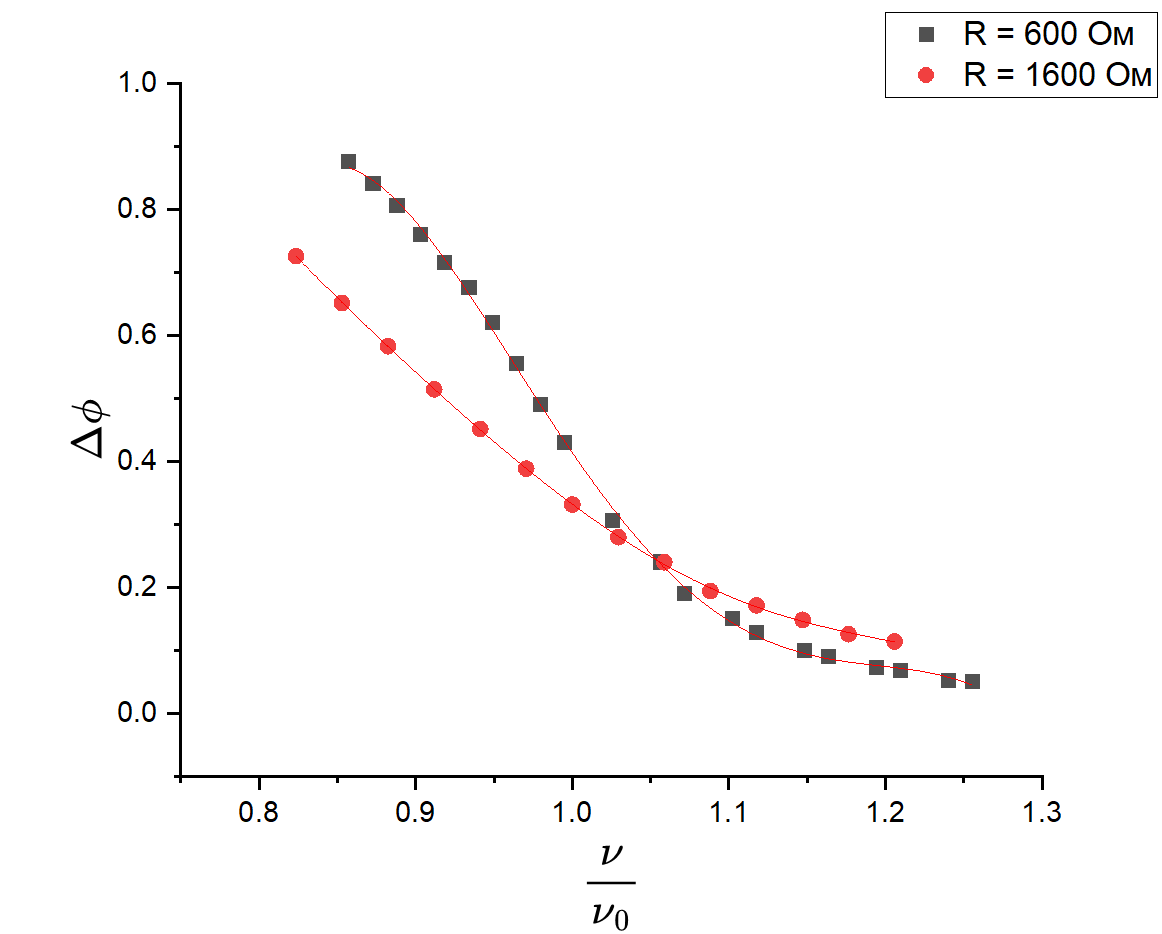
\includegraphics[width=\textwidth]{G5.png}
\caption{Фазово-частотная характеристика} \label{G5}
\end{center}
\end{figure}

\begin{figure}[H]
\begin{center}
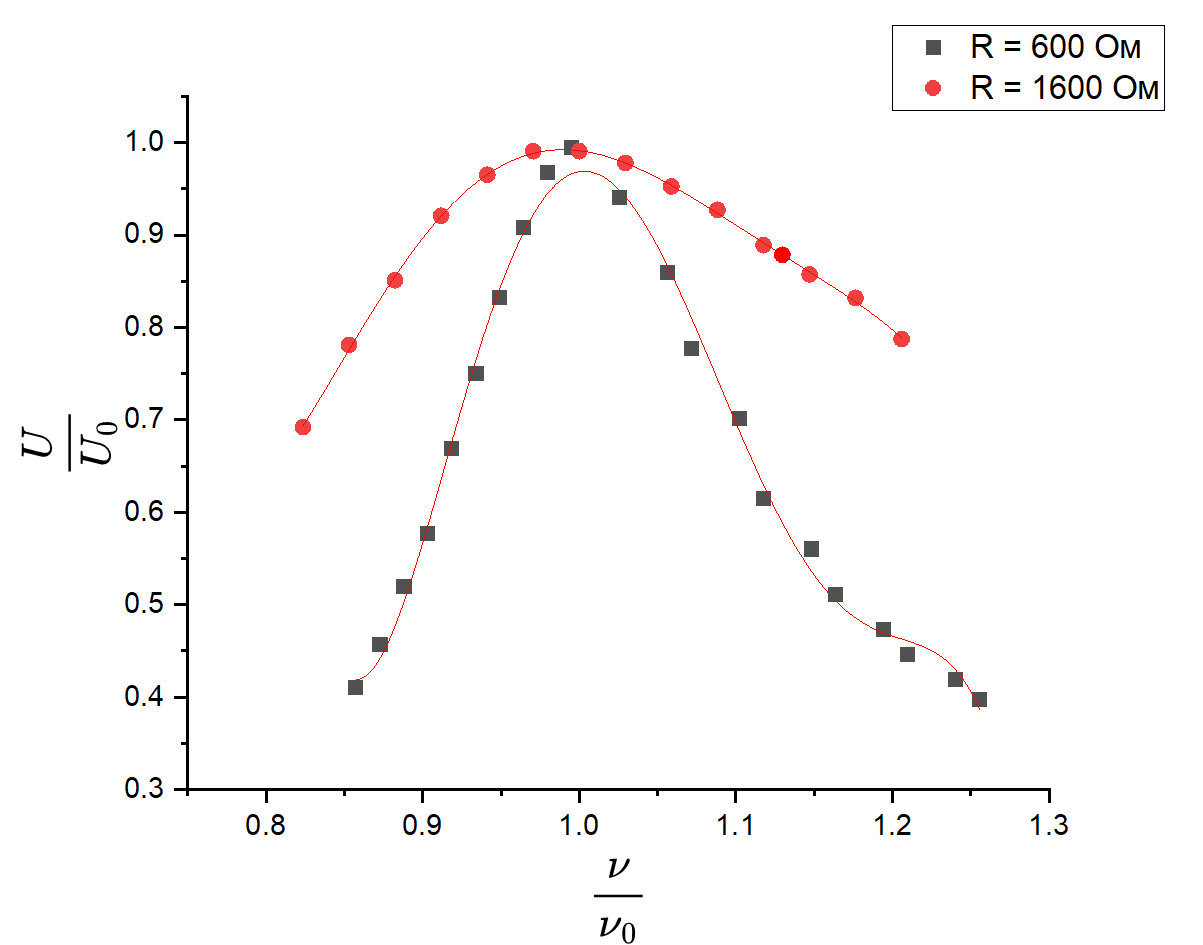
\includegraphics[width=\textwidth]{G4.png}
\caption{Амплитудно-частотная характеристика} \label{G4}
\end{center}
\end{figure}



\subsection{Нахождение добротности контура}

\textbf{1.} Рассчитаем добротность контура $Q = \pi/\Theta$ для максимального и минимального значения $\Theta$ по спирали на фазовой кривой:

$$Q = \pi/\Theta$$
$$\sigma_Q = Q \cdot \frac{\sigma_\Theta}{\Theta}$$

При $R = 600$ Ом: $Q = (6,6 \pm 0,4)$
При $R = 1600$ Ом: $Q = (2,5 \pm 0,3)$

\textbf{2.} Теоретическое значение добротности через параметры $L$, $C$, $R$:

$$Q = \frac{1}{R}\sqrt{\frac{L}{C}}$$

При $R = 600$ Ом: $Q = 6,8$
При $R = 1600$ Ом: $Q = 2,6$

\textbf{3.} Рассчитаем добротность контура по АЧХ по формуле:

$$Q = \frac{\nu_0}{2\Delta\Omega}$$
$$\sigma_Q = Q \frac{\sigma_\Delta}{\Delta\Omega}, \;\; \sigma_\Delta = 0,1 \text{ Гц}$$
где $\Omega$ --- ширина резонансной кривой, измеренная на уровне $\nu_0/\sqrt{2}$

При $R = 600$ Ом: $Q = (6,6 \pm 0,1)$
При $R = 1600$ Ом: $Q = (2,5 \pm 0,1)$

\textbf{4.} Рассчитаем добротность по ФЧХ. Отметим горизонтальной линией уровень, соответствующий разности фаз $-\pi/2$. Зеркально отразим нижнюю часть зависимости относительно проведенной горизонтальной линии. Измерим $\Delta \Omega$ на уровне $-\pi/4$. Добротность контура вычисляется по формуле:
$$Q = \frac{\omega_0}{\Delta \Omega}$$
$$\sigma_Q = Q \sqrt{ \lr{\frac{\sigma_\omega}{\omega}}^2 + \lr{\frac{\sigma_\Delta}{\Delta \Omega}}^2 }, \;\; \sigma_\omega = 0,3 \text{ Гц}, \sigma_\Delta = 0,3 \text{ Гц}$$

При $R = 600$ Ом: $Q = (6,0 \pm 0,4)$
При $R = 1600$ Ом: $Q = (2,0 \pm 0,4)$

Занесём в таблицу полученные данные добротности для $R = 600$ Ом и $R = 1600$ Ом:

\begin{table}[H]
\centering
\caption{Измерение добротности колебаний в контуре}
\label{tab:5}
\begin{tabular}{|c|c|c|c|c|}
\hline
              & $f(L, C, R)$ & Спираль     & АЧХ             & ФЧХ             \\ \hline
$R = 600$ Ом  & 6,8          & $(6,6 \pm 0,4)$ & $(6,6 \pm 0,1)$ & $(6,0 \pm 0,4)$ \\ \hline
$R = 1600$ Ом & 2,6          & $(2,5 \pm 0,3)$ & $(2,5 \pm 0,1)$ & $(2,0 \pm 0,4)$ \\ \hline
\end{tabular}
\end{table}


\textbf{6.} Измерим активное сопротивление $R_L$ и индуктивность $L$ магазина индуктивностей с помощью измерителя LCR на частотах 50 Гц, 500 Гц и 1500 Гц. Результаты занесём в таблицу

\begin{table}[H]
\centering
\caption{Измерение активного сопротивления и индуктивности магазина.}
\label{tab:5}
\begin{tabular}{|c|c|c|}
\hline
$\nu$, Гц & L, мкГн & R, Ом \\ \hline
50    & 1       & 0,72  \\ \hline
500   & 0,8     & 0,718 \\ \hline
1500  & 0,77    & 0,716 \\ \hline
\end{tabular}
\end{table}


\section{ Вывод}
\begin{enumerate}
    \item Были исследованы свободные и вынужденные колебания в контуре.
    \item Наблюдали характерные зависимости этих колебаний от времени на экране осциллографа.
    \item Сняты АЧХ и ФЧХ контура для двух значений сопротивления.
    \item Получены параметры схемы, такие как $R_{cr}$ и $\Theta$.
\end{enumerate}
\newpage
\begin{figure}[H]
	\begin{center}
	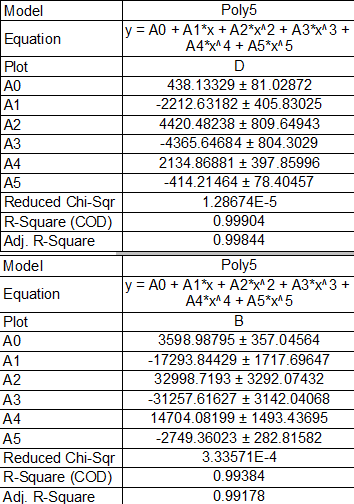
\includegraphics[width=\textwidth]{G6.png}
	\end{center}
	\end{figure}
	\begin{figure}[H]
	\begin{center}
	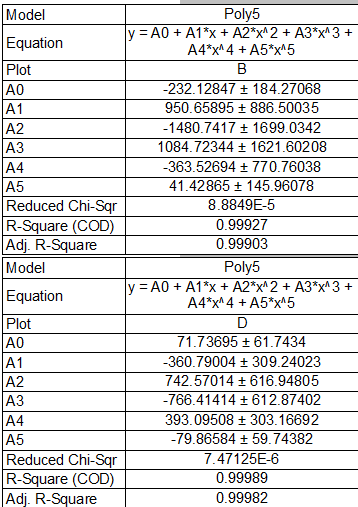
\includegraphics[width=\textwidth]{image2.png}
	\end{center}
	\end{figure}
\end{document}